\PhanI
%\loai{Chu kì}
\begin{ex}%[3P1BF-2][Loai1]
Một con lắc đơn có chiều dài 1 m, dao động điều hòa tại nơi có gia tốc trọng trường $g = 9,8\ m/s^2$. Chu kì dao động của con lắc là
\choice
{1,99 s}
{2,00 s}
{\True 2,01 s}
{1 s}
\loigiai{
Ta có: $T = 2\pi \sqrt {\dfrac{\ell}{g}} = 2\pi \sqrt {\dfrac{1}{9,8}} = 2,007\ s$.
}
%\haidong{2}
\end{ex} \haidong{20}
%\loai{Tần số}
\begin{ex} %[3P1BF-2][Loai1]  
Một con lắc đơn dao động điều hòa theo phương trình $s=2\cos \left({\pi t+\dfrac{\pi }{3}}\right)$ cm. Tần số dao động của con lắc đơn này là
\choice
{\True 0,5 Hz}
{1 Hz}
{4 Hz}
{2 Hz}
\loigiai{
Tần số dao dộng của con lắc là $f=\dfrac{\omega }{2\pi}=\dfrac{\pi }{2\pi}=0,5\ Hz$.
}

%\haidong{4}
\end{ex} \haidong{20}
\begin{ex} %[3P1BF-2][Loai1]  
Một con lắc đơn có chiều dài dây treo là 64 cm. Lấy $g=\pi ^2\ m/s^2$. Số dao động toàn phần vật thực hiện được trong 24 giây là
\choice
{\True 15}
{10}
{1,5}
{25}
\loigiai{
\begin{itemize}
\item Chu kì dao động của con lắc $T=2\pi \sqrt{\dfrac{\ell}{g}}=2\pi \sqrt{\dfrac{0,64}{10}}=1,6\ s.$
\item Mỗi chu kì vật thực hiện được một dao động toàn phần $\Rightarrow $ khoảng thời gian $\Delta t=15T=24\ s \Rightarrow $ vật thực hiện được 15 dao động toàn phần.
\end{itemize}
}
%\haidong{6}
\end{ex} \haidong{20}

%\loai{Xác định gia tốc rơi tự do}
\begin{ex}%[3P1KF-2][Loai1]
Một con lắc đơn dao động điều hoà tại địa điểm A với chu kì 2 s. Đưa con lắc này tới địa điểm B cho nó dao động điều hoà, trong khoảng thời gian 201 s nó thực hiện được 100 dao động toàn phần. Coi chiều dài dây treo của con lắc đơn không đổi. Gia tốc trọng trường tại B so với tại A
\choice
{tăng 0,1\%}
{tăng 1\%}
{\True giảm 1\%}
{giảm 0,1\%}
\loigiai{
$\begin{cases}
2\ s = 2\pi \sqrt{\dfrac{\ell}{g_A}} \\
\dfrac{201}{100} = 2\pi \sqrt {\dfrac{\ell}{g_B}} 
\end{cases} 
\Rightarrow \dfrac{2,01}{2} = \sqrt {\dfrac{g_A}{g_B}} \Rightarrow g_B = 0,99g_A = 99\% {g_A}$ 
$\Rightarrow$ giảm 1\%.
}
%\haidong{7}
\end{ex} \haidong{20}
%\loai{Chu kì thay đổi do thay đổi chiều dài}
\begin{ex}%[3P1KF-2][Loai1]
Tại một nơi trên mặt đất, con lắc đơn có chiều dài $\ell$ đang dao động điều hòa với chu kì 2 s. Khi tăng chiều dài của con lắc thêm 21 cm thì chu kì dao động điều hòa của nó là 2,2 s. Chiều dài $\ell$ bằng
\choice
{2 m}
{\True 1 m}
{2,5 m}
{1,5 m}
\loigiai{
Ta có: $\begin{cases}
2\ s = 2\pi \sqrt {\dfrac{\ell}{g}} \\2,2\ s =2\pi \sqrt {\dfrac{\ell + 0,21}{g}} \end{cases} \Rightarrow \dfrac{2}{2,2} = \sqrt {\dfrac{\ell}{\ell + 0,21}} \Rightarrow \ell = 1\ m$.
}
%\haidong{4}
\end{ex} \haidong{20}

\begin{ex}%[3P1KF-2][Loai1]
Tại một nơi trên mặt đất, một con lắc đơn dao động điều hoà. Trong khoảng thời gian  $\Delta t$ , con lắc thực hiện 40 dao động toàn phần; thay đổi chiều dài con lắc một đoạn 7,9 cm thì cũng trong khoảng thời gian  $\Delta t$  ấy, nó thực hiện 39 dao động toàn phần. Chiều dài của con lắc sau khi thay đổi là
\choice
{\True 160 cm}
{152,1 cm}
{144,2 cm}
{167,9 cm}
\loigiai{Ta có
\begin{align*}
\left.\begin{array}{l}
\dfrac{{\Delta t}}{{40}}= 2\pi\sqrt{\dfrac{\ell}{g}}\\
\dfrac{{\Delta t}}{{39}}=2\pi\sqrt{\dfrac{{\ell\pm 0,079}}{g}}
\end{array}\right\}\Rightarrow\dfrac{{39}}{{40}}=\sqrt{\dfrac{\ell}{{\ell\pm 0,079}}}\Rightarrow\dfrac{{39}}{{40}}=\sqrt{\dfrac{\ell}{{\ell\pm 0,079}}}\Rightarrow\ell = 152,1\ cm\Rightarrow\ell ' = 160\ cm.
\end{align*}
}
%\haidong{6}
\end{ex} \haidong{20}


%\loai{Chu kì thay đổi do thay đổi chiều dài - mối quan hệ tỉ lệ}


\begin{ex}%[3P1KF-2][Loai1] 
Một con lắc đơn gồm quả nặng có khối lượng m và dây treo có chiều dài $\ell$ có thể thay đổi được. Nếu chiều dài dây treo là $\ell_1$ thì chu kì dao động của con lắc là 1 s. Nếu chiều dài dây treo là $\ell_2$ thì chu kì dao động của con lắc là 2 s. Nếu chiều dài con lắc là $\ell_3= 4\ell_1+ 3\ell_2$ thì chu kì dao động của con lắc là
\choice
{\True 4 s}
{6 s}
{5 s}
{3 s}
\loigiai{
\begin{itemize}
\item 
\begin{align*}
T\sim \sqrt{\ell}\xrightarrow{{\ell_3=4\ell_1+3\ell_2}}{T}_3=\sqrt{4T_1^2+3T_2^2}=4\ s.
\end{align*}
\item 
\end{itemize}
}
%\haidong{9}
\end{ex} \haidong{20}



%\loai{\% Chu kì thay đổi}
\begin{ex}%[3P1KF-2][Loai1]
Một con lắc đơn có chiều dài 120 cm. Để chu kì dao động giảm 10\% thì chiều dài dây treo con lắc phải
\choice
{tăng 22,8 cm}
{\True giảm 22,8 cm}
{tăng 18,9 cm}
{giảm 97,2 cm}
\loigiai{
\begin{itemize}
\item $\begin{cases}T = 2\pi \sqrt {\dfrac{{1,2}}{g}} \\90\% T=2\pi \sqrt {\dfrac{\ell '}{g}} \end{cases} \Rightarrow \dfrac{10}{9} = \sqrt {\dfrac{1,2}{\ell '}} \Rightarrow \ell ' = 97,2\ cm.$
\item Vậy phải giảm đi $120 - 97,2 = 22,8$ cm.
\end{itemize}
}
%\haidong{7}
\end{ex} \haidong{20}

\begin{ex} %[3P1BF-2][Loai1]  
Để chu kì của con lắc đơn tăng thêm 4\% thì phải tăng chiều dài của nó thêm
\choice
{8\%}
{16\%}
{\True 8,16\%}
{4\%}
\loigiai{
\begin{itemize}
\item Ta có: $\left\{ \begin{aligned} &T = 2\pi.\sqrt{\dfrac{\ell}{g}}\\ 
&1,04T = 2\pi.\sqrt{\dfrac{\ell'}{g}}\\
\end{aligned}\right.$\\
$\Rightarrow 1,04 = \sqrt{\dfrac{\ell'}{\ell}}$
$\Rightarrow \ell' = 108,16\%\ell$
$\Rightarrow$ Chiều dài dây treo tăng thêm 8,16\%.

\end{itemize}}

%\haidong{8}
\end{ex} \haidong{20}



%\loai{Hai con lắc}






%\loai{Công thức độc lập}
\begin{ex} %[3P1-16.3][Loai1]  
Một con lắc đơn có chiều dài $\ell = 1$ m được kéo ra khỏi vị trí cân bằng một góc $\alpha _0=5^\circ$ so với phương thẳng đứng rồi thả nhẹ cho vật dao động. Cho $g=\pi ^2=10\ m/s^2$. Tốc độ của con lắc khi về đến giá trị cân bằng là
\choice
{15,8 m/s}
{\True 0,278 m/s}
{0,028 m/s}
{0,087 m/s}
\loigiai{
Vận tốc con lắc khi qua vị trí cân bằng:  $v_{\max}=\omega.S_0=\sqrt{\dfrac{g}{\ell}}.\ell.\alpha_0=0,278$ m/s.
}
%\haidong{3}
\end{ex} \haidong{20}

\begin{ex}%[3P1KF-3][Loai1] 
Con lắc đơn chiều dài 1 m dao động nhỏ với chu kì 1,5 s và biên độ góc là 0,05 rad. Khi li độ góc bằng 0,04 rad thì tốc độ của vật là
\choice
{$9\pi $ cm/s}
{$3\pi $ cm/s}
{\True $4\pi $ cm/s}
{$\dfrac{4\pi}{3}$ cm/s}
\loigiai{Độ lớn vận tốc khi vật có li độ góc 0,04 rad
\begin{align*}
\begin{cases}
T=2\pi \sqrt{\dfrac{\ell}{g}}\Rightarrow g=\dfrac{4\pi ^2\ell}{T^2}
\\
v^2=g\ell\left(\alpha_0^2-\alpha ^2\right)=\dfrac{4\pi ^2\ell^2}{T^2}\left(\alpha_0^2-\alpha ^2\right)\Rightarrow \left|v\right|=0,04\pi \ m/s\\ 
\end{cases}
\end{align*}
}
%\haidong{3}
\end{ex} \haidong{20}
\begin{ex} %[3P1-16.3][Loai1]  
Một con lắc đơn dao động điều hòa với biên độ góc 0,1 rad ở một nơi có gia tốc trọng trường $g = 10\ m/s^2$. Vào thời điểm ban đầu vật đi qua vị trí có li độ dài 8 cm và có tốc độ $20\sqrt{3}\ cm/s$. Tốc độ cực đại của vật dao động là
\choice
{0,8 m/s}
{0,2 m/s}
{\True 0,4 m/s}
{1 m/s}
\loigiai{
Áp dụng công thức độc lập thời gian, ta có:
\begin{align*}
S_0^2=s^2+\dfrac{v^2}{\omega ^2}\Leftrightarrow &\left(\ell \alpha_0\right)^2=s^2+\dfrac{\ell.v^2}{g}\\
\Leftrightarrow &\left(\ell.0,1\right)^2=0,08^2+\dfrac{\ell.0,04.3}{10}\Rightarrow \ell=1,6\ m
\Rightarrow v_{\max}=\omega S_0=\sqrt{\dfrac{g}{\ell}}.\ell \alpha_0=0,4\ m/s.
\end{align*}
}
%\haidong{4}
\end{ex} \haidong{20}
\begin{ex}%[3P1BF-2][Loai1]%Bài 18
Một con lắc đơn dao động điều hoà với biên độ góc $\alpha_0 = 0,1$ rad tại nơi có gia tốc $g = 10\ m/s^2$. Tại thời điểm ban đầu, vật đi qua vị trí có li độ dài $s=8\sqrt{3}\ cm$ với tốc độ $v = 20$ cm/s. Chiều dài dây treo vật là
\choice
{80 cm}
{100 cm}
{\True 160 cm}
{120 cm}
\loigiai{
\begin{itemize}
\item Ta có: $s=\ell \alpha \Rightarrow \alpha =\dfrac{s}{\ell}=\dfrac{0,08\sqrt{3}}{\ell}$.
\item $\alpha _0^2=\alpha^2+\dfrac{v^2}{g\ell}\Rightarrow 0,1^2=\dfrac{\left( 0,08\sqrt{3}\right)^2}{\ell^2}+\dfrac{0,2^2}{10\ell}\Rightarrow \ell =-1,2\ m$ hoặc $\ell =1,6\ m$.
\end{itemize}
}
%\haidong{4}
\end{ex} \haidong{20}

\begin{ex}%[3P1-16.3K][Loai1] 
Vật treo của con lắc đơn dao động điều hòa theo cung tròn $\widearc{MN}$ quanh vị trí cân bằng O. Gọi P và Q lần lượt là trung điểm của $\widearc{MO}$ và $\widearc{MP}$. Biết vật có tốc độ cực đại 8 m/s. Tốc độ của vật khi đi qua Q là
\choice
{6 m/s}
{\True 5,29 m/s}
{3,46 m/s}
{8 m/s}
\loigiai{Áp dụng công thức độc lập thời gian, ta có
\begin{align*}
1=\left(\dfrac{s}{S_0}\right)^2+\left(\dfrac{v}{\omega S_0}\right)^2\xrightarrow{|x_Q|=\frac{3S_0}{4}}\left|v\right|=\omega S_0.\sqrt{1-\dfrac{9}{16}}\approx 5,29\ m/s.
\end{align*}}
%\haidong{4}
\end{ex} \haidong{20}
%\loai{Động năng}
\begin{ex}%[3P1-16.3K][Loai1] 
Một con lắc đơn gồm một viên bi nhỏ khối lượng 100 g được treo ở đầu một sợi dây dài 1,57 m tại địa điểm có gia tốc trọng trường $9,81\ m/s^2$. Kéo con lắc lệch khỏi vị trí cân bằng một góc 0,1 rad rồi thả cho nó dao động điều hoà không có vận tốc ban đầu. Động năng viên bi khi góc lệch của nó là 0,05 rad là
\choice
{$W_{\text{đ}} = 0,00195$ J}
{$W_{\text{đ}} = 0,00585$ J}
{$W_{\text{đ}} = 0,00591$ J}
{\True $W_{\text{đ}} = 0,00577$ J}
\loigiai{Động năng viên bi khi góc lệch của nó là 0,05 rad:
\begin{align*}
W_{\text{đ}}=W-W_t=\dfrac{mg\ell}{2}\alpha_0^2-\dfrac{mg\ell}{2}\alpha^2=0,00577\ J.
\end{align*}}
%\haidong{4}
\end{ex} \haidong{20}
%\loai{Thế năng và động năng}


\begin{ex}%[3P1-16.3K][Loai1]
Một con lắc đơn ($m = 200$ g, $\ell =$ 80 cm) treo tại nơi có $g = 10$ $m/s^2$. Kéo con lắc lệch khỏi vị trí cân bằng góc $\alpha_0$ rồi thả không vận tốc đầu, con lắc dao động điều hoà với năng lượng $W = 3,2.10^{-4}$ J. Biên độ dao động là
\choice
{$S_0 = 3$ cm}
{$S_0= 2$ cm}
{$S_0= 1,8$ cm}
{\True $S_0= 1,6$ cm}
\loigiai{
\begin{itemize}
\item Ta có công thức tính năng lượng của con lắc đơn dao động điều hòa: 
\begin{align*}
W = \dfrac{mgS^2_0}{2\ell}\Rightarrow S_0 = \sqrt{\dfrac{2E\ell}{mg}} = 0,016\ m = 1,6\ cm.
\end{align*}
\end{itemize}
}
%\haidong{4}
\end{ex} \haidong{20}

%\loai{Viết phương trình dao động}
\begin{ex} %[3P1BF-4][Loai1]  
Một con lắc đơn đang dao động điều hòa với biên độ góc bằng $0,05\pi \ rad$ dưới tác dụng của trọng lực. Ở thời điểm ban đầu, dây treo con lắc lệch khỏi phương thẳng đứng góc bằng $0,025\pi \ rad$ và vật đang chuyển động về vị trí cân bằng theo chiều âm với tốc độ $\dfrac{{\sqrt{75}}}{2}\pi ^2 \ cm/s.$ Lấy $g=\pi ^2\ m/s^2.$ Phương trình dao động của vật là
\choice
{$\alpha =0,05\pi \cos\left(4\pi t+\dfrac{\pi }{3}\right)\ rad$}
{$\alpha =0,05\pi \cos\left(\pi t-\dfrac{2\pi}{3}\right)\ rad$}
{$\alpha =0,05\pi \cos\left(2\pi t+\dfrac{2\pi}{3}\right)\ rad$}
{\True $\alpha =0,05\pi \cos\left(\pi t+\dfrac{\pi }{3}\right)\ rad$}
\loigiai{
\begin{itemize}
\item Thời điểm ban đầu con lắc đang ở vị trí có li độ $\alpha =\dfrac{\alpha _0}{2}$ và đang chuyển động theo chiều âm $\Rightarrow \varphi=\dfrac{\pi }{3}$.
\item Áp dụng công thức độc lập giữa biên độ dài, li độ và vận tốc, ta có:
\begin{align*}
\left(\ell \alpha _0\right)^2=\left(\ell \alpha\right)^2+\left(\dfrac{v}{\sqrt{\dfrac{g}{\ell}}}\right)=1\Leftrightarrow \ell=\dfrac{v^2}{g\left(\alpha _0^2-\alpha ^2\right)}=0,1\ m \Rightarrow \omega =\pi.
\end{align*}
\end{itemize}
}
%\haidong{4}
\end{ex} \haidong{20}
\begin{ex}%[3P1-15.4K][Loai1]%Bài 18
Một con lắc đơn có chiều dài dây treo $\ell  = 20$ cm dao động tại nơi có $g = 9,8\ m/s^2$. Ban đầu người ta kéo vật lệch khỏi phương thẳng đứng một góc 0,1 rad rồi truyền cho vật tốc độ 14 cm/s phương vuông góc với dây treo hướng về vị trí cân bằng. Chọn gốc thời gian lúc truyền tốc độ, chiều dương là chiều kéo lệch vật thì phương trình li độ dài của vật là
\choice
{$s=2\sqrt{2}\cos  \left( 7t-\dfrac{\pi}{4} \right)\ cm$}
{\True $s=2\sqrt{2}\cos  \left( 7t+\dfrac{\pi}{4} \right)\ cm$}
{$s=2\sqrt{2}\cos  \left( 7t+\dfrac{3\pi}{4} \right)\ cm$}
{$s=2\sqrt{2}\cos  \left( 7t-\dfrac{3\pi}{4} \right)\ cm$}
\loigiai{
\begin{itemize}
\item Ta có: $\alpha _0^2=\alpha^2+\dfrac{v^2}{g\ell}\Rightarrow \alpha_0=0,1\sqrt{2}\ rad \Rightarrow s_0 = \ell.\alpha_0 = 2\sqrt{2}\ cm$.
\item Tại $t = 0:\ \alpha =\dfrac{\alpha_0\sqrt{2}}{2}\ (-)\Rightarrow \varphi =\dfrac{\pi}{4}$.
\end{itemize}
}
%\haidong{5}
\end{ex} \haidong{20}
\PhanII
\setcounter{ex}{0}
\begin{ex}
Một con lắc đơn có chiều dài $\ell = 1\ m$, khối lượng $m = 0,1\ kg$, kéo lệch $10^\circ$ rồi thả nhẹ. Tại $t = 0$, vật đi qua vị trí cân bằng theo chiều dương. Lấy $g=\pi^2 = 10\ m/s^2$.
\choiceTF[t]
{Biên độ góc của dao động là $10\ rad$}
{Chu kì của dao động là $4\ s$}
{\True Tần số góc của dao động là $\pi\ rad/s$}
{\True Phương trình li độ góc là $\alpha = \dfrac{\pi}{18} \cos(\pi t - \dfrac{\pi}{2})\ rad$}
\loigiai{
\begin{itemchoice}
\itemch $\alpha_0 = 10^\circ = \dfrac{\pi}{18}\ rad$
\itemch $T = 2\pi\sqrt{\dfrac{1}{g}} = 2\ s$
\itemch $\omega = \dfrac{2\pi}{T} = \pi\ rad/s$
\itemch Vì đi qua VTCB theo chiều dương nên $\varphi = -\dfrac{\pi}{2}$
\end{itemchoice}
}
\end{ex}
\begin{ex}
Con lắc đơn dao động điều hòa với chu kì $4 \ s$. Biết quỹ đạo vật có chiều dài $20 \ cm$. Lấy $g=\pi^2\ m/s^2$.
\choiceTF[t]
{Chiều dài dây là $1 \ m$}
{Biên độ dài của dao động là $4\ cm$}
{\True Biên độ góc dao động là $0,025\ rad$}
{Tốc độ cực đại của vật trong quá trình dao động là $\pi\ m/s$}
\loigiai{
\begin{itemchoice}
\itemch
\itemch
\itemch
\itemch
\end{itemchoice}
}
%\haidong{6}
\end{ex} \haidong{20}
\begin{ex}
Một con lắc đơn có độ dài dây treo là $1\ m$ và treo quả nặng $1\ kg$, kéo con lắc lệch khỏi vị trí cân bằng góc $0,1\ rad$ rồi buông nhẹ. Chọn thời điểm ban đầu vật ở biên âm. Lấy $g=\pi^2=10\ m/s^2$.
\choiceTF[t]
{Con lắc có phương trình li độ dài $s = 10\cos(\pi t)\ cm$}
{\True Thế năng của con lắc được tính theo công thức \linebreak $W_t = mg\ell(1 - \cos\alpha)$}
{Khi con lắc chuyển động với tốc độ bằng một nửa tốc độ cực đại thì động năng xấp xỉ $0,025\ J$}
{Khi con lắc chuyển động tới vị trí có li độ dài $s = 5\ cm$ thì con lắc có thế năng bằng động năng}
\loigiai{
\begin{itemchoice}
\itemch Sai do thiếu pha ban đầu, đúng là $s = 10\cos(\pi t - \pi)$.
\itemch Đúng, là công thức chuẩn xác cho thế năng con lắc đơn.
\itemch Sai, khi $v = v_{max}/2$, động năng là $0,0125\ J$.
\itemch Sai, vì khi $s = A/2$, ta có $W_t = \dfrac{1}{4}W \Rightarrow W_d = \dfrac{3}{4}W$.
\end{itemchoice}
}
\end{ex}
\begin{ex}
Tại nơi có $g = 10\ m/s^2$, một con lắc đơn dao động điều hòa với phương trình $\alpha = 0,1 \cos \left(2\pi t + \dfrac{\pi}{3}\right)$ rad.
\choiceTF[t]
{\True Tần số của con lắc phụ thuộc vào chiều dài dây treo và gia tốc trọng trường}
{Chu kì của con lắc là $T = 0,5\ s$}
{\True Tốc độ của con lắc khi dây treo thẳng đứng là $v_{\max} = \dfrac{1}{2\pi}\ m/s$}
{\True Tại thời điểm $t = 2\ s$, li độ góc của con lắc là $0,05\ rad$}
\loigiai{
\begin{itemchoice}
\itemch $f = \dfrac{1}{2\pi} \sqrt{\dfrac{g}{\ell}}$ nên phụ thuộc cả $g$ và $\ell$
\itemch $\omega = 2\pi \Rightarrow T = \dfrac{2\pi}{2\pi} = 1\ s$
\itemch $v_{\max} = \omega \alpha_0 \ell = \alpha_0 \dfrac{g}{\omega} = 0,1 \cdot \dfrac{10}{2\pi} = \dfrac{1}{2\pi}\ m/s$
\itemch $\alpha(2) = 0,1 \cos(4\pi + \dfrac{\pi}{3}) = 0,1 \cos \dfrac{\pi}{3} = 0,05\ rad$
\end{itemchoice}
}
\end{ex}
\PhanIII
\setcounter{ex}{0}
\begin{ex}
Một con lắc đơn có chiều dài dây treo $\ell_1$ dao động với biên độ góc nhỏ và chu kì dao động là $T_1=0,6 \ s$. Con lắc đơn có chiều dài $\ell_2$ có chu kì dao động cũng tại nơi đó là $T_2=0,8 \ s$. Chu kì của con lắc có chiều dài $\ell=\ell_1+\ell_2$ là bao nhiêu giây?
\shortans[oly]{1} \loigiai{
1
}
%\haidong{7}
\end{ex} \haidong{20}
\begin{ex}
Tại một nơi, chu kì dao động điều hoà của một con lắc đơn là $2,0 \ s$. Sau khi tăng chiều dài của con lắc thêm $21 \ cm$ thì chu kì dao động điều hoà của nó là $2,2 \ s$. Chiều dài ban đầu của con lắc này là bao nhiêu cm?
\shortans[oly]{100}
\loigiai{
100
}
%\haidong{7}
\end{ex} \haidong{20}
\begin{ex}
Một con lắc đơn đang dao động điều hòa với biên độ góc $9^\circ$ dưới tác dụng của trọng lực. Ở thời điểm $t_0$, vật nhỏ của con lắc có li độ góc và li độ cong lần lượt là $4,5^\circ$ và $2,5 \pi\ cm$. Lấy $g=10 \ m/s^2$. Tốc độ của vật ở thời điểm $t_0$ là bao nhiêu $cm/s$ (làm tròn kết quả đến chữ số hàng phần mười)?
\shortans[oly]{4,3}
\loigiai{
4,3
}
%\haidong{7}
\end{ex} \haidong{20}
\begin{ex}%[3P1-16.3K][Loai1] 
Một con lắc đơn có khối lượng $2\ kg$ và có độ dài $4\ m$, dao động điều hòa ở nơi có gia tốc trọng trường $9,8\ m/s^2$. Cơ năng dao động của con lắc là $0,2205\ J$. Biên độ góc của con lắc bằng bao nhiêu độ (làm tròn kết quả đến chữ số hàng phần mười)?
\shortans[oly]{4,3}
\loigiai{Biên độ góc của con lắc
\begin{align*}
W=\dfrac{mg\ell}{2}\alpha_0^2\Rightarrow \alpha_0=\sqrt{\dfrac{2W}{mg\ell}}=\sqrt{\dfrac{2.0,2205}{2.9,8.4}}=0,075\ rad=4,3\degree.
\end{align*}}
\end{ex} \haidong{20}
\begin{ex}
\immini[thm]{Trong bài thực hành đo gia tốc trọng trường $g$ bằng con lắc đơn, một nhóm học sinh tiến hành đo, xử lý số liệu và vẽ được đồ thị biểu diễn sự phụ thuộc của bình phương chu kì dao động điều hòa $\left(T^2\right)$ theo chiều dài $\ell$ của con lắc như hình bên.  Lấy $\pi=3,14$. Giá trị trung bình của $g$ đo được trong thí nghiệm này là bao nhiêu $m/s^2$ (làm tròn kết quả đến chữ số hàng phần trăm)?}{\begin{tikzpicture}[draw=Mapcolor,scale=1,thick,>=stealth']
\tkzDefPoints{0/0/o, 4/0/x, 0/4/y}
\draw  [help  lines, xstep=0.5cm,ystep=0.5cm]  (0,0)  grid  (3.45,3.45);
\tkzDrawSegments[->](o,x o,y)
\node[below] at (0.5,0) {$0,3$};
\node[left] at (0,0.5) {$0,81$};
\tkzLabelPoint[below](x){$\ell\ (m)$}
\tkzLabelPoint[above](y){$T^2\ (s^2)$}
\tkzLabelPoint[below left](o){$O$}
\draw[Mapcolor,dashed,thin] (0,0) -- (2.2,3.3);
\draw[Mapcolor,very thick] (0.6,0.9) -- (2.2,3.3);
\draw[fill=Mapcolor,Mapcolor!50] (0.55,1.1) -- (0.55,1) -- (0.65,1) -- (0.65,1.1) -- (0.55,1.1);
\draw[fill=Mapcolor,Mapcolor!50]  (0.95,1.55) -- (0.95,1.45) -- (1.05,1.45) -- (1.05,1.55) -- (0.95,1.55);
\draw [fill=Mapcolor,Mapcolor!50] (1.4,2.1) -- (1.4,2) -- (1.5,2) -- (1.5,2.1) -- (1.4,2.1);
\draw [fill=Mapcolor,Mapcolor!50] (1.6,2.6) -- (1.6,2.5) -- (1.7,2.5) -- (1.7,2.6) -- (1.6,2.6);
\draw[fill=Mapcolor,Mapcolor!50]  (1.95,3.05) -- (1.95,2.95) -- (2.05,2.95) -- (2.05,3.05) -- (1.95,3.05);
\end{tikzpicture}}

\shortans[oly]{9,74}
\loigiai{
9,74
}
%\haidong{8}
\end{ex} \haidong{20}
\begin{ex}
\immini[thm]{
Một con lắc đơn lớn được treo ở sảnh của toà nhà Liên Hợp Quốc tại thành phố New York, Mỹ có gia tốc rơi tự do $g=9,81\ m/s^2$. Quả cầu có khối lượng 91 kg và sợi dây treo dài 22,9 m. Con lắc liên tục dao động với chu kì 9,6 s. Khi con lắc liên tục dao động với biên độ $8^\circ$ gần như không đổi. Bỏ qua lực cản. Cơ năng của con lắc là bao nhiêu jun (làm tròn kết quả đến chữ số hàng phần trăm)?
}{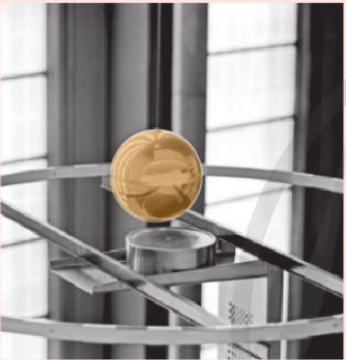
\includegraphics[width=4cm]{Hinh/CDLHQ}}
\shortans[oly]{8,69} 
\loigiai{
\begin{itemize}
\item Cơ năng của con lắc là: $W=mg\ell.\left(1-\cos\alpha_0\right)=91.9,81.22,9(1-\cos 8^\circ)=8,688\ J$.
\end{itemize}
}
%\haidong{4}
\end{ex} \haidong{20}












